\documentclass{uwstat572}

%%\setlength{\oddsidemargin}{0.25in}
%%\setlength{\textwidth}{6in}
%%\setlength{\topmargin}{0.5in}
%%\setlength{\textheight}{9in}

\renewcommand{\baselinestretch}{1.5} 
\usepackage{amsmath}
\usepackage{bm}
\usepackage{subfigure}
\usepackage{amsmath}    % allows AMS math things like the cases environment
\usepackage{amssymb}    % allows the use of AMS symbols like blackboard bold
\usepackage{amsthm}     % allows AMS definitions for theorems, proofs, etc.
\usepackage{graphicx}   % need for figures
 \usepackage{epsfig}
\usepackage{verbatim}   % useful for program listings
\usepackage{color}      % use if color is used in text
\usepackage{subfigure}  % use for side-by-side figures
\usepackage{morefloats}
\usepackage{float}
\usepackage[font={small}]{caption}

\bibliographystyle{plainnat}

\begin{document}
%%\maketitle

\begin{center}
  {\LARGE Forecasting Time Series With Complex Seasonal Patterns Using Exponential Smoothing  }\\\ 
  {\large Alysha M. De Livera, Rob J. Hyndman, and Ralph D. Synder}\\\ \\
  {Mengjie Pan \\ 
    Department of Statistics, University of Washington Seattle, WA, 98195, USA
  }
\end{center}


%\begin{abstract}
%  Put your project summary here.
%\end{abstract}

\section{Introduction}


\begin{figure}[]
\minipage{\textwidth}
  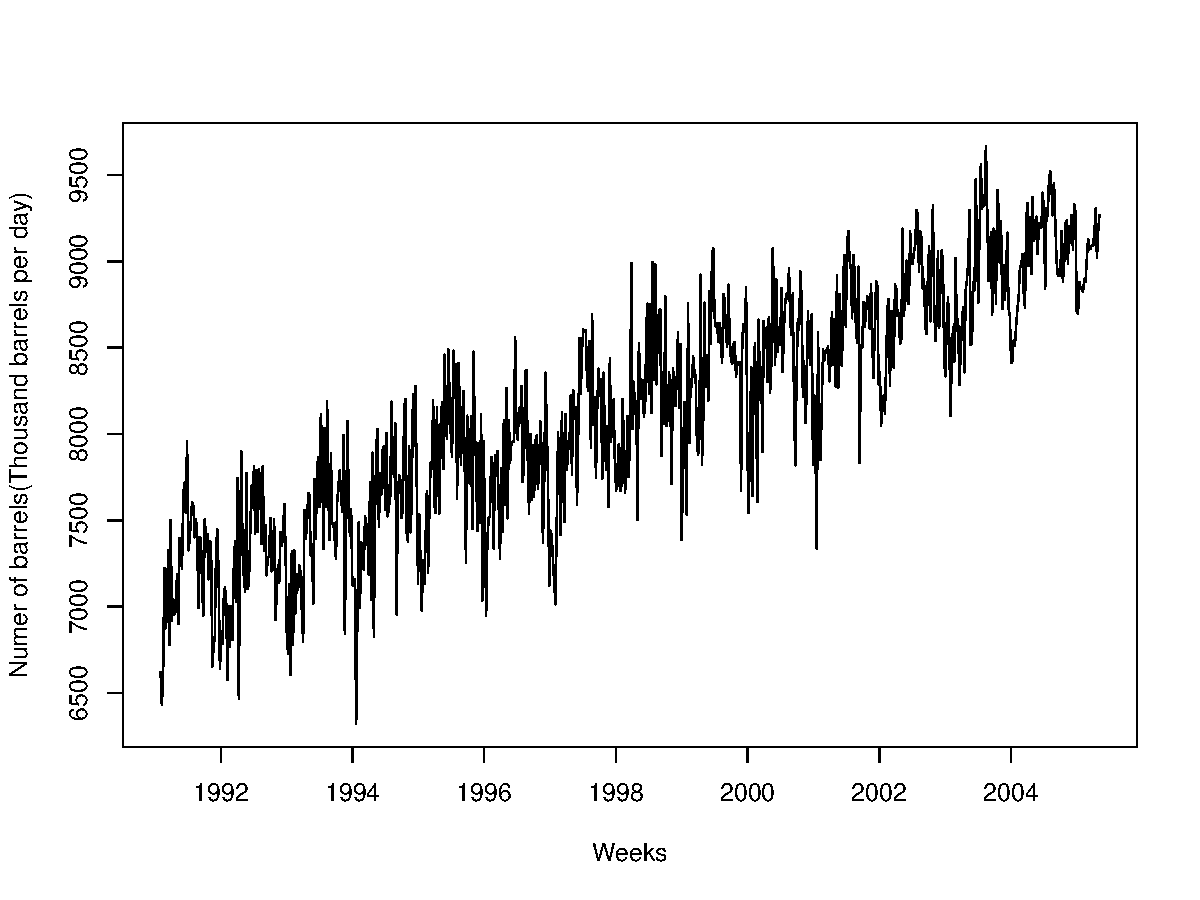
\includegraphics[width=6in,height=2.7in]{gas}
\endminipage\hfill
\minipage{\textwidth}
  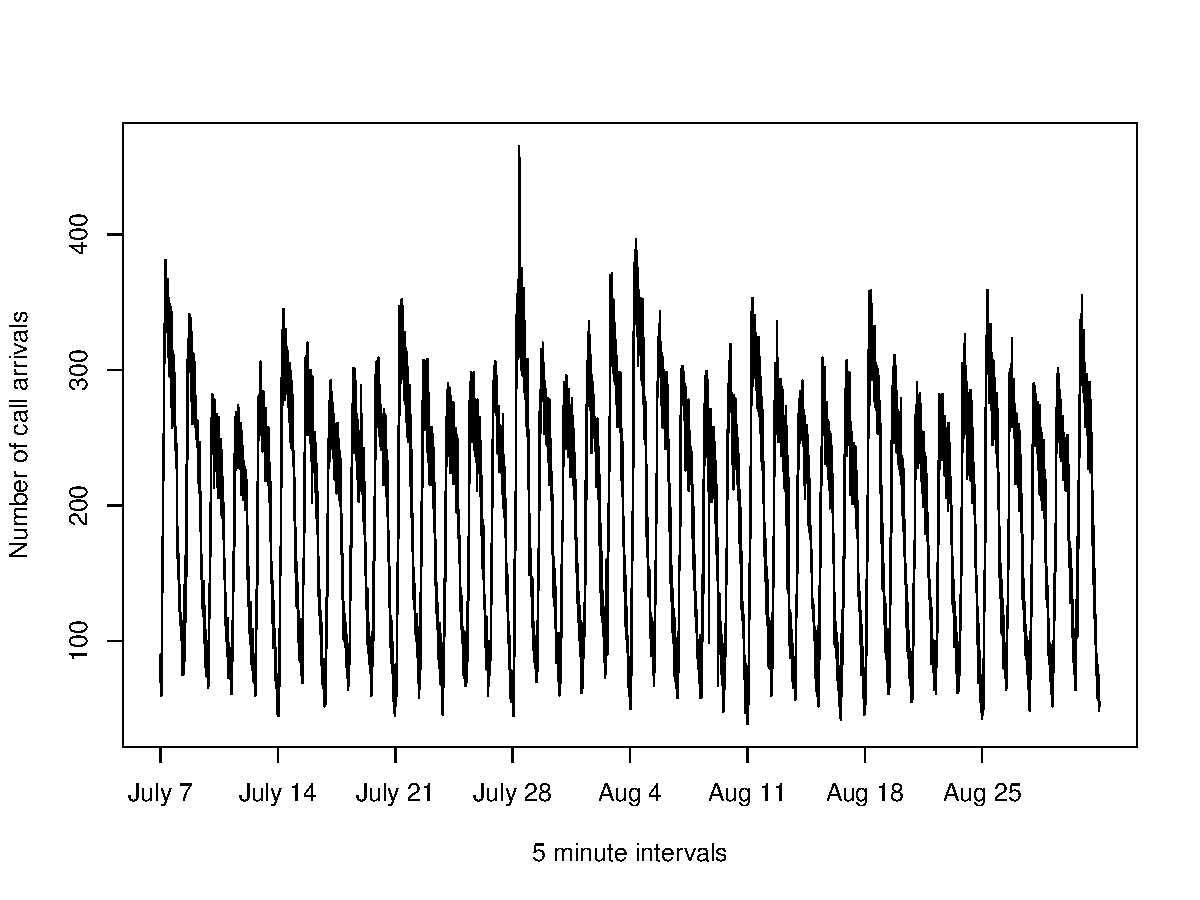
\includegraphics[width=6in,height=2.7in]{calls}
\endminipage\hfill
\minipage{\textwidth}
  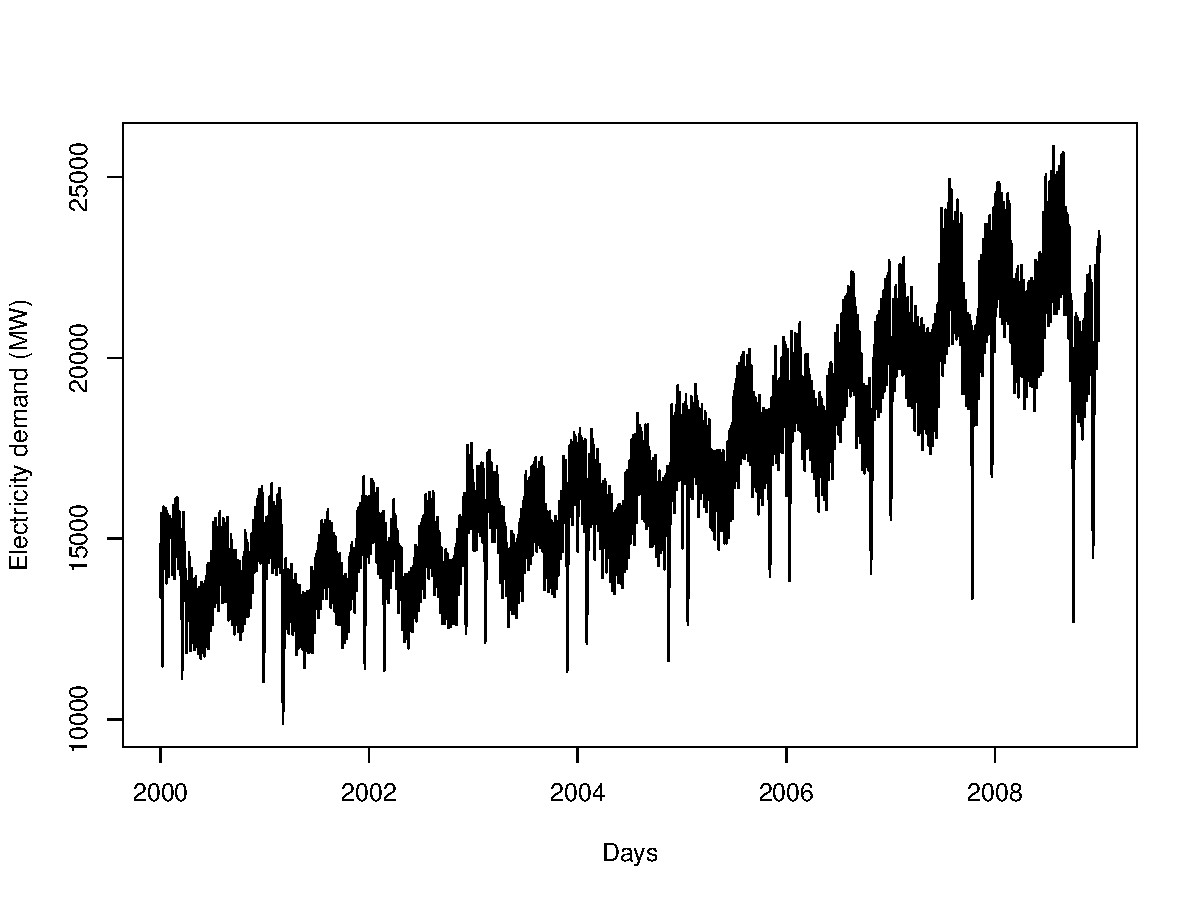
\includegraphics[width=6in,height=2.7in]{telec}
\endminipage
\caption{Plots of three time series datasets used in this report (from top to bottom): U.S finished motor gasoline products supplied from February 1991 to July 2005, number of call arrivals handled on weekdays between 7 a.m. and 9:0.5 p.m from July 7, 2003, to August 29, 2003 in a bank, Turkish electricity demand data from January 1, 2000, to December 31, 2008.}
\label{fig:data}
\end{figure}

\hspace{4ex}Many time series have complex seasonal patterns, such as non-integer seasonal periods, multiple nested and non-nested seasonal periods. For example, a weekly series of U.S. gasoline products supplied has an annual seasonal pattern with a non-integer period of 365.25/7 $\approx 52.18$. A five-minute interval series of number of call arrivals in a commercial bank has a daily seasonal pattern and a weekly seasonal pattern, which is an example of multiple nested seasonal periods. We also provide an example of non-integer and multiple non-nest seasonal periods: a daily series of the electricity demand in Turkey is affected by events on the Hijri calendar of a period of 354.37 and the Gregorian calendar of a period of 365.25, and therefore has two annual seasonal patterns whose periods are approximately eleven days apart. Figure \ref{fig:data} shows the plots of all three datasets considered in this report.

A number of existing approaches deal with some of the above complexities. \citet{pedregal2006modulated}, \citet{harvey1993forecasting} and \citet{taylor2003short} considered double seasonality, and \citet{taylor2010triple} considered triple seasonality. \citet{harvey1997modeling} used single trigonometric seasonality to deal with a non-integer seasonal period. However, none of the previous methods allows for non-integer seasonal periods and multiple seasonal periods at the same time, and therefore cannot be applied to Turkish electricity demand time series. To remedy this shortcoming, \citet{de2011forecasting} propose two new state space models that use exponential smoothing. 

We now present some literature on the development of forecasting models using exponential smoothing. Simple exponential smoothing calculates forecasts using weighted averages of observed time series, where the weights decrease exponentially as observations becomes further in the past. \citet{holt1957forecasting} and \citet{winters1960forecasting} extended simple exponential smoothing to include trend and seasonality components in the model. \citet{hyndman2002state} discussed a class of innovations state space models, where `innovations' refers to a single source of error. The innovations state space framework allows for trend, seasonality and error specification of forecasting models. The Holt-Winters additive and multiplicative methods are specific cases of the framework with an additive trend. One of the most commonly used single seasonal models in the framework is the linear version of the Holt-Winters method with additive errors:

\begin{subequations}
\begin{align}
 y_t=&l_{t-1}+b_{t-1}+s_{t-m_1}^{(1)}+d_t, \label{eqn:measurement.simple}\\
 l_t=&l_{t-1}+b_{t-1}+\alpha d_t,\label{eqn:level.simple} \\
 b_t=&b_{t-1}+\beta d_t,\label{eqn:trend.simple} \\
 s_t^{(1)}=&s_{t-m_1}^{(1)}+\gamma d_t,\label{eqn:error.simple}
\end{align}
\label{eqn:simple}
\end{subequations}

\noindent where $\{y_t\}$ is the time series, $m_1$ is the period of the seasonal pattern, $\{d_t\}$ is a series of uncorrelated white-noise random variable, $l_t, b_t, s_t$ represent the level, trend and seasonal components at time $t$, and $\alpha,\beta,\gamma$ are smoothing parameters.

One problem is that this model does not allow for non-integer periods and multiple seasonal periods. More seasonal components can be added to this model, ($s_t^{(2)},...,s_t^{(T)}$); however, a large number of initial states ($l_0, b_0, \{ s^{(1)}_{1-m_1}, ..., s_0^{(1)} \},...,  \{ s^{(T)}_{1-m_T}, ..., s_0^{(T)} \}$) need to be estimated when one of the seasonal patterns has large periods. \citet{taylor2003short}, \citet{taylor2010triple}, and \citet{gould2008forecasting} approximated initial seasonal values with various heuristic approaches, but their methods were not statistically principled. Another problem is that the above model assumes that the elements of the error process $\{d_t\}$ is uncorrelated, but there is empirical evidence that they might be correlated (\citet{taylor2003short}). A further problem is that the nonlinear version of state space models can have infinite forecast variances (\citet{akram2009exponential}). 

To accommodate non-integer seasonal periods and multiple seasonal periods, \citet{de2011forecasting} propose two innovations state space models using exponential smoothing, BATS, and TBATS. BATS is an acronym for features of the model: Box-Cox transformation, autoregressive moving average (ARMA) errors, Trend, and Seasonal components. Box-Cox transformation is employed to allow some nonlinearity, yet to avoid the problem with nonlinear models mentioned above. An ARMA process is used to allow for correlation of errors. TBATS is an extension of BATS that is based on trigonometric formulation of seasonal components, with the initial T standing for ``trigonometric". The benefits of trigonometric formulation are the ability to have non-integer seasonal periods and significant decrease of the number of initial states. 

\citet{de2011forecasting} introduce a new state space modeling framework, which includes the two new models they propose. They present an estimation algorithm using the state space formulation, which returns least squares estimates of initial states and maximum likelihood estimates of parameters. With estimated parameters and initial states, they can obtain point forecasts and forecast intervals using inverse Box-Cox transformation of quantiles of the prediction distribution. We reproduced the proposed models and  applied them to all three datasets of U.S. gasoline supply, number of call arrivals, and electricity demand in Turkey. We evaluated our forecasts from our proposed models using the root mean squared error (RMSE), and we compared BATS forecasts with TBATS forecasts.

\section{Methods}
\subsection{BATS Model}
%\hspace{4ex}To deal with the problems with nonlinear models and correlated errors and allow for multiple seasonal periods, \citet{de2011forecasting} propose a BATS model. BATS model adds a Box-Cox transformation and more seasonal periods to model \ref{eqn:simple} and replace white noise errors with ARMA errors. 

\hspace{4ex}A BATS$( \omega, \phi, p, q, m_1, m_2, ..., m_T )$ model is given by:  

\begin{subequations}
\begin{align}
y_t^{  (w)} = &\left\{
\begin{array}{l l}
\frac{y_t^{w}-1}{w}, & if \;\; w \neq 0,\\
\log y_t, & if\;\; w=0,\\
\end{array} \right. \\
y_t^{  (w)}=&l_{t-1}+\phi b_{t-1} +\sum\limits_{i=1}^T s_{t-m_i}^{(i)}+d_t, \label{eqn:measurement} \\
l_t=&l_{t-1}+\phi b_{t-1}+\alpha d_t,\label{eqn:level}  \\
 b_t=&\phi b_{t-1}+\beta d_t, \label{eqn:trend} \\
 s_t^{(i)}=&s_{t-m_i}^{(i)}+\gamma_i d_t, \label{eqn:seasonal} \\
 d_t=&\sum\limits_{i=1}^p \varphi_id_{t-i} +\sum\limits_{i=1}^q \theta_i \epsilon_{t-i}+\epsilon_t, \\
 \epsilon_t &  \stackrel{iid}{\sim} N(0,\sigma^2),
\end{align}
\end{subequations}
\noindent where $m_1,..., m_T$ denote the seasonal periods, $l_t$ and $b_t$ are the level and trend components at time $t$, $s_t^{(i)}$ represents the $i$th seasonal component at time $t$, and $d_t$ denotes ARMA(p,q) process. Parameters $\alpha, \beta, \gamma_i, i=1,...,T$ are smoothing parameters, and $\phi$ is a damping parameter. Equation \ref{eqn:measurement} is usually referred to as the measurement equation, and Equations \ref{eqn:level}-\ref{eqn:seasonal} are usually referred to as transition (level, trend, seasonal respectively) equations as they describe how the unobserved components or states change over time. 

BATS model reduces to model defined by Equations \ref{eqn:simple} when $\omega=1$, $\phi=1$, $p=q=0$ and $T=1$, so the model in \ref{eqn:simple} is given by BATS$(1,1,0,0, m_1)$. Compared to the model defined by Equations \ref{eqn:simple}, BATS model has more flexibility for fitting time series data since it has the option of including a Box-Cox transformation and ARMA errors. However, depending on the actual dataset, the BATS model with non-trivial $\omega, p, q$ may be less preferable compared to simple models, such as the model in \ref{eqn:simple}. A model selection procedure, proposed by  \citet{de2011forecasting}, with appropriate orders $p$ and $q$ and with inclusion of non-trivial Box-Cox parameter or damping parameter is described in Section \ref{sec:selection}. 

The seasonal part of the measurement equation is $\sum\limits_{i=1}^T s_{t-m_i}^{(i)}$, which does not make sense when $m_i$ is not an integer. Another disadvantage of BATS model is that the number of initial states to be estimated is $\sum\limits_{i=1}^T m_i$, which could be large if at least one $m_i$ is large. To fix these two problems, \citet{de2011forecasting} propose TBATS model, which we describe in the next section.  

\subsection{TBATS Model}
\hspace{4ex}The main distinction between BATS and TBATS models is that the TBATS model is based on trigonometric formulation of seasonal components, thus allowing for non-integer seasonal periods. The seasonal part of the measurement equation needs to adjust with this change correspondingly. A TBATS $(\omega, \phi, p, q, \{m_1,k_1\}, \{m_2,k_2\},...,\{m_T,k_T\} )$ is given by:

\begin{subequations}
\begin{align}
%y_t^{  (w)} =& \left\{
%\begin{array}{l l}
%\frac{y_t^{w}-1}{w}, & if \;\; w \neq 0,\\
%\log y_t, & if\;\; w=0,\\
%\end{array} \right. \\
y_t^{  (w)}=&l_{t-1}+\phi b_{t-1} +\sum\limits_{i=1}^T s_{t-1}^{(i)}+d_t, \\
%l_t=&l_{t-1}+\phi b_{t-1}+\alpha d_t, \\
 %b_t=&\phi b_{t-1}+\beta d_t, \\
s_t^{(i)}=&\sum\limits_{j=1}^{k_i} s_{j,t}^{(i)},\;\;  \lambda_{j}^{(i)}=2\pi j /m_i \\
s_{j,t}^{(i)}=&s_{j,t-1}^{(i)} \cos \lambda_j^{(i)} + s_{j,t-1}^{*(i)} \sin \lambda_j^{(i)} +\gamma_1^{(i)}d_t, \\
s_{j,t}^{*(i)}=&-s_{j,t-1}^{(i)} \sin \lambda_j^{(i)} + s_{j,t-1}^{*(i)} \cos \lambda_j^{(i)} +\gamma_2^{(i)}d_t. \\
% d_t=&\sum\limits_{i=1}^p \varphi_id_{t-i} +\sum\limits_{i=1}^q \theta_i \epsilon_{t-i}+\epsilon_t, \\
 %\epsilon_t & \stackrel{iid}{\sim} N(0,\sigma^2),
\end{align}
\end{subequations}
\noindent where $m_1,..., m_T$ denote the seasonal periods and $s_t^{(i)}$ represents the $i$th seasonal component at time $t$. The Box-Cox equation, level and trend equations, and ARMA errors equation remain the same as in BATS. In the trigonometric formulation of seasonal components, $k_i$ is the number of harmonics for $i$th seasonal component, $s_{j,t}^{(i)}$ is the stochastic level of the $i$th seasonal component, and$s_{j,t}^{*(i)}$ is the stochastic growth in the level of the $i$th seasonal component. Parameters $\alpha, \beta, \gamma_i, i=1,...,T$ are smoothing parameters, and $\phi$ is a damping parameter. 

The number of initial states to be estimated is $2\sum\limits_{i=1}^T k_i$. If we take $k_i=m_i/2$ for even numbers of $m_i$ or $k_i=(m_i-1)/2$ for odd numbers of $m_i$, the number of estimated initial states will be approximately equal to that of BATS model. However, it is anticipated that most seasonal components require fewer than $m_i/2$ harmonics. 

The TBATS model resolves both of the problems of the BATS model while retaining its advantages: the TBATS model allows for non-integer seasonal periods and multiple seasonal periods, and significantly decreases the number of estimated initial states. It is necessary to select the number of harmonics $k_i$ and orders $p$ and $q$ before we fit a TBATS model to data. The model selection procedure will be described in Section \ref{sec:selection}.

\subsection{Innovations State Space Formulations}
\hspace{4ex}\citet{de2011forecasting} introduce a new linear innovations state space modeling framework to include the Box-Cox transformation, with BATS and TBATS as special cases of the framework. One benefit of the innovations state space formulation is that we can easily work with this general formulation when we estimate parameters and make forecasts. The linear innovations state space model has the form:

\begin{subequations}
\begin{align}
y_t^{  (w)}=&\textbf{w}'\textbf{x}_{t-1}+\epsilon_t, \label{eqn:innov1}\\
\textbf{x}_t=&\textbf{Fx}_{t-1}+\textbf{g}\epsilon_t, \label{eqn:innov2}
\end{align}
\end{subequations}
\noindent where $\textbf{w}'$ is a row vector, $\textbf{x}_t$ is the unobserved state vector at time $t$, \textbf{F} is a matrix, \textbf{g} is a column vector, and $\epsilon_t$ is the error term. Equation \ref{eqn:innov1} is referred to as the measurement equation, and Equation \ref{eqn:innov2} is referred to as the transition equation.

\subsubsection{BATS Model}
\hspace{4ex}The state vector of the BATS model is $\textbf{x}_t=(l_t,b_t,\textbf{s}_t^{(1)},...,\textbf{s}_t^{(T)}, d_t, d_{t-1},..., d_{t-p+1}, \epsilon_t, \epsilon_{t-1},\\ \epsilon_{t-q+1} )'$, 
where $\textbf{s}_t^{(i)}=(s_t^{(i)}, s_{t-1}^{(i)} ,..., s_{t-(m_i-1)}^{(i)}  )$. Let $\bm{\gamma}^{(i)}$=$(\gamma_i, \textbf{0}_{m_i-1})$, $\bm{\gamma}=(\bm{\gamma}^{(1)},\bm{\gamma}^{(2)},...,\bm{\gamma}^{(T)})$, $\bm{\varphi}=(\varphi_1, \varphi_2,..., \varphi_p)$, and $\bm{\theta}=(\theta_1,\theta_2,...,\theta_q)$; let $\textbf{O}_{u,v}$ be a $u \times v$ matrix of zeros, let $\textbf{I}_{u,v}$ be a $u \times v$ rectangular diagonal matrix with element 1 on the diagonal, and let $\textbf{a}^{(i)}=(\textbf{0}_{m_i-1},1)$ and $\textbf{a}=(\textbf{a}^{(1)},...,\textbf{a}^{(T)})$. We define the matrices $\textbf{B}=\bm{\gamma}'\bm{\varphi}, \textbf{C}=\bm{\gamma}'\bm{\theta}$, $\textbf{A}_i=\begin{bmatrix} 
\textbf{0}_{m_i-1} &1 \\ 
\textbf{I}_{m_i-1} & \textbf{0}'_{m_i-1} 
\end{bmatrix}$ and $\textbf{A}=\oplus _{i=1}^T \textbf{A}_i$, where $\oplus$ denotes the direct sum of the matrices. Let $\tau=\sum_{i=1}^{T} m_i$. 
Then the matrices for the BATS model can be written as $\textbf{w}=(1,\phi,\textbf{a}, \bm{\varphi}, \bm{\theta})' \in \mathbf{R}^{2+\tau+p+q}$, \textbf{g}=$(\alpha,\beta,\bm{\gamma}, 1, \textbf{0}_{p-1}, 1, \textbf{0}_{q-1})'\in \mathbf{R}^{2+\tau+p+q}$, and 

\begin{center}
$\textbf{F}=\begin{bmatrix} 
1 & \phi& \textbf{0}_\tau & \alpha \bm{\varphi} & \alpha \bm{\theta}  \\
0 & \phi& \textbf{0}_\tau & \beta \bm{\varphi} & \beta \bm{\theta}  \\
\textbf{0}'_\tau &  \textbf{0}'_\tau  & \bm{A} & \bm{B} & \bm{C} \\
0 & 0 & \textbf{0}'_\tau & \bm{\varphi} & \bm{\theta}  \\
\bm{0}'_{p-1} & \bm{0}'_{p-1} & \textbf{O}_{p-1,\tau} & \bm{I}_{p-1,p} &\textbf{O}_{p-1,q} \\
0 & 0 &\textbf{0}_\tau & \textbf{0}_p & \textbf{0}_q \\
\bm{0}'_{q-1} & \bm{0}'_{q-1} & \textbf{O}_{q-1,\tau} & \bm{I}_{q-1,p} &\textbf{O}_{q-1,q} \\
\end{bmatrix} \in \mathbf{R}^{(2+\tau+p+q) \times (2+\tau+p+q)}$ 
\end{center}

\vspace{2mm} \noindent This is the general formulation with all components present. When one component is not present, the corresponding row and/or column must be omitted. For example, in the absence of a trend component, the second row in $\textbf{g}, \textbf{w}$ and $\textbf{F}$ must be omitted. 

\subsubsection{TBATS Model}
\hspace{4ex}The innovations state space formulation of the TBATS model is similar to one of the BATS model but has changes in $\textbf{s}_t^{(i)}, \textbf{a}^{(i)}, \bm{\gamma}^{(i)}, \tau$ and $\textbf{A}$ due to trigonometric representation of seasonal components. The state vector of the TBATS model is $\textbf{x}_t=(l_t,b_t,\textbf{s}_t^{(1)},...,\textbf{s}_t^{(T)}, d_t, d_{t-1},\\..., d_{t-p+1},  \epsilon_t, \epsilon_{t-1}, \epsilon_{t-q+1} )'$, 
where $\textbf{s}_t^{(i)}=(s_{1,t}^{(i)},s_{2,t}^{(i)},..., s_{1,k-_i}^{(i)}, s_{1,t}^{*(i)},s_{2,t}^{*(i)},...,s_{k_i,t}^{*(i)})$. 
Let $\textbf{1}_r$ and $\textbf{0}_r$ be one-vector and zero-vector of length $r$, respectively; let $\bm{\gamma}_1^{(i)}=\gamma_1^{(i)} \textbf{1}_{k_i}, \bm{\gamma}_2^{(i)}=\gamma_2^{(i)} \textbf{1}_{k_i}, \bm{\gamma}^{(i)}$=$(\bm{\gamma}_1^{(i)},\\ \bm{\gamma}_2^{(i)})$, $\bm{\gamma}=(\bm{\gamma}^{(1)},\bm{\gamma}^{(2)},...,\bm{\gamma}^{(T)})$, $\bm{\varphi}=(\varphi_1, \varphi_2,..., \varphi_p)$, and $\bm{\theta}=(\theta_1,\theta_2,...,\theta_q)$; let $\textbf{O}_{u,v}$ be a $u \times v$ matrix of zeros, let $\textbf{I}_{u,v}$ be a $u \times v$ rectangular diagonal matrix with element 1 on the diagonal, and let $\textbf{a}^{(i)}=(\textbf{1}_{k_i},\textbf{0}_{k_i})$ and $\textbf{a}=(\textbf{a}^{(1)},...,\textbf{a}^{(T)})$. We define the matrices $\textbf{B}=\bm{\gamma}'\bm{\varphi}, \textbf{C}=\bm{\gamma}'\bm{\theta}$, $\textbf{A}_i=\begin{bmatrix} 
\textbf{C}^{(i)} &\textbf{S}^{(i)}  \\ 
-\textbf{S}^{(i)}  &\textbf{C}^{(i)} 
\end{bmatrix}$ and $\textbf{A}=\oplus _{i=1}^T \textbf{A}_i$, where $\textbf{C}^{(i)}$ and $\textbf{S}^{(i)}$ are $k_i \times k_i$ diagonal matrices with entries $\cos (\lambda^{(i)}_j) $, $\sin (\lambda^{(i)}_j) $, respectively, for $j=1,2,...,k_i$ and $i=1,2,...,T$, and where $\oplus$ denotes the direct sum of the matrices. Let $\tau=2\sum_{i=1}^{T} k_i$. 

Then the matrices for the TBATS model can be written as $\textbf{w}=(1,\phi,\textbf{a}, \bm{\varphi}, \bm{\theta})' \in \mathbf{R}^{2+\tau+p+q}$, \textbf{g}=$(\alpha,\beta,\bm{\gamma}, 1, \textbf{0}_{p-1}, 1, \textbf{0}_{q-1})'\in \mathbf{R}^{2+\tau+p+q}$, and 

\begin{center}
$\textbf{F}=\begin{bmatrix} 
1 & \phi& \textbf{0}_\tau & \alpha \bm{\varphi} & \alpha \bm{\theta}  \\
0 & \phi& \textbf{0}_\tau & \beta \bm{\varphi} & \beta \bm{\theta}  \\
\textbf{0}'_\tau &  \textbf{0}'_\tau  & \bm{A} & \bm{B} & \bm{C} \\
0 & 0 & \textbf{0}'_\tau & \bm{\varphi} & \bm{\theta}  \\
\bm{0}'_{p-1} & \bm{0}'_{p-1} & \textbf{O}_{p-1,\tau} & \bm{I}_{p-1,p} &\textbf{O}_{p-1,q} \\
0 & 0 &\textbf{0}_\tau & \textbf{0}_p & \textbf{0}_q \\
\bm{0}'_{q-1} & \bm{0}'_{q-1} & \textbf{O}_{q-1,\tau} & \bm{I}_{q-1,p} &\textbf{O}_{q-1,q} \\
\end{bmatrix} \in \mathbf{R}^{(2+\tau+p+q) \times (2+\tau+p+q)}$ 
\end{center}

\noindent Same as the BATS formulation, when one component is not present, the corresponding row and/or column must be omitted.

\subsubsection{ARIMA Reduced Forms}
The linear innovations state space models have equivalent ARIMA reduced forms. The reduced forms of BATS and TBATS are summarized and delivered in Section 2.4.3 in \citet{de2011forecasting} and the proofs are presented in \citet{dethesis}. Because the rest of the paper does not rely on ARIMA reduced forms, we do not go into detail in this report. 

\subsection{Estimation Algorithm}
In this section we derive the likelihood of the observed time series $\textbf{y}=(y_1,y_2,...,y_n)$ and present an estimation algorithm proposed by \citet{de2011forecasting} for estimating initial states and parameters, based on the innovations state space formulation. The Kalman filter is typically used to obtain one-step-ahead prediction errors; in this paper, initial states are treated as fixed parameters, and both the parameters and initial parameters are selected to maximize the conditional likelihood. The measurement equation \ref{eqn:innov1}, with the assumption of $\epsilon_t \sim N(0,\sigma^2)$, implies $y_t^{(\omega)} \sim N(\textbf{w}'\textbf{x}_{t-1},\sigma^2)$. The Jacobian of the Box-Cox transformation is

\begin{center}
$\displaystyle \frac{\partial y_t^{(\omega)}}{ \partial  y_t }= \left\{
\begin{array}{l l}
y_t^{\omega-1}, & if \;\; w \neq 0\\
1/ y_t, & if\;\; w=0\\
\end{array} \right. =y_t^{\omega-1}\;\;  \forall \omega,$ 
\end{center}
so
\begin{align*}
\displaystyle P(y_t| \textbf{x}_{t-1}, \bm{\nu},\sigma^2)&=P(y_t^{(\omega)}| \textbf{x}_{t-1}, \bm{\nu},\sigma^2) \left| \det\left( \frac{\partial y_t^{(\omega)}}{ \partial  y_t }   \right) \right| \\
&= P(y_t^{(\omega)}| \textbf{x}_{t-1}, \bm{\nu},\sigma^2) y_t^{\omega-1},
\end{align*}
where $\bm{\nu}$ is a vector containing Box-Cox parameter $\omega$, smoothing parameters ($\alpha,\beta$, $\bm{\gamma}$), damping parameter $\phi$, and ARMA coefficients ($\bm{\varphi}$, $\bm{\theta}$). The joint distribution is
\begin{align*}
\displaystyle P(\textbf{y}| \textbf{x}_0, \bm{\nu},\sigma^2)&= \prod\limits_{t=1}^n P(y_t|y_1,...,y_{t-1},\textbf{x}_0, \bm{\nu},\sigma^2) \\
&= \displaystyle   \prod\limits_{t=1}^n P(y_t|\textbf{x}_{t-1}, \bm{\nu},\sigma^2)
= \displaystyle   \prod\limits_{t=1}^n  P(y_t^{(\omega)}| \textbf{x}_{t-1}, \bm{\nu},\sigma^2) y_t^{\omega-1} \\
&=\displaystyle   \prod\limits_{t=1}^n P(\epsilon_t)  \prod\limits_{t=1}^n y_t^{\omega-1}
=\displaystyle \frac{1}{(2\pi \sigma^2)^{n/2}} \exp \left(  \frac{-1}{2\sigma^2}  \sum\limits_{t=1}^n \epsilon_t^2 \right)   \prod\limits_{t=1}^n y_t^{\omega-1},
\end{align*}

\noindent which gives the log likelihood
\begin{equation}
\mathcal{L}(\textbf{x}_0, \bm{\nu},\sigma^2)=-\frac{n}{2} \log (2\pi \sigma^2) -\frac{1}{2\sigma^2} \sum\limits_{t=1}^n \epsilon_t^2 +(\omega-1) \sum\limits_{t=1}^n \log(y_t).
\label{eqn:loglik}
\end{equation}

\noindent where $\epsilon_t=y_t^{(\omega)}-\textbf{w}' \sum\limits_{j=1}^{t-1} \textbf{D}^{j -1}\textbf{g} y_{t-j} -\textbf{w}' \textbf{D}^{t-1} \textbf{x}_0$ and $\textbf{D}=\textbf{F}-\textbf{g} \textbf{w}'$ (discussed in detail below). Although $\bm{\nu}$ does not show up explicitly in the likelihood function \ref{eqn:loglik}, elements in $\bm{\nu}$ are used to construct \textbf{w}, \textbf{g}, \textbf{F}, and \textbf{D}. Plugging in the maximum likelihood estimate of variance $\hat{\sigma^2}=n^{-1} \sum\limits_{t=1}^n \epsilon_t^2$ into Equation \ref{eqn:loglik}, dropping constant terms and multiplying by $-2$, we get

\begin{equation}
\mathcal{L}^{*}(\textbf{x}_0, \bm{\nu})=n \log (\sum\limits_{t=1}^n \epsilon_t^2)-2(\omega-1) \sum\limits_{t=1}^n \log(y_t).
\label{eqn:objective}
\end{equation}

Our objective is to find maximum likelihood estimates, and equivalently to minimize likelihood in Equation \ref{eqn:objective}. One challenge is that when the number of initial states is large, there are too many values to be optimized. To reduce the number of parameters in the numerical optimization problem, \citet{de2011forecasting} propose to concentrate the initial state out of the likelihood. The idea is to write errors $\epsilon_t$ as a linear function of initial states $\textbf{x}_0$ and then use least squares to estimate $\textbf{x}_0$. Under the innovations state space formulation, the transition Equation \ref{eqn:innov2} is equivalent to 
\begin{equation}
\textbf{x}_t=\textbf{D}\textbf{x}_{t-1}+\textbf{g}y_t^{(\omega)}, \label{eqn:backsolve}
\end{equation}
where $\textbf{D}=\textbf{F}-\textbf{g} \textbf{w}'$. To see why this holds, we substitute $\displaystyle  \epsilon_t=y_t^{(\omega)}-\textbf{w}'\textbf{x}_{t-1}$ into the transition equation \ref{eqn:innov2} and we get
\begin{align*}
\textbf{x}_t&= \textbf{F}\textbf{x}_{t-1}+\textbf{g}(y_t^{(\omega)}-\textbf{w}'\textbf{x}_{t-1}) \\
&= (\textbf{F}-\textbf{g} \textbf{w}') \textbf{x}_{t-1} +\textbf{g} y_t^{(\omega)} \\
&= \textbf{D} \textbf{x}_{t-1} +\textbf{g}y_t^{(\omega)}  .
\end{align*}
Then we can back-solve the recurrence equation \ref{eqn:backsolve} to get 
\begin{center}
$\textbf{x}_t=\textbf{D}^t \textbf{x}_0+\sum\limits_{j=0}^{t-1} \textbf{D}^j \textbf{g} y_{t-j}$.
\end{center}
Thus we have 
\begin{align*}
\epsilon_t &= y_t^{(\omega)}-\textbf{w}'\textbf{x}_{t-1} \\
&= y_t^{(\omega)}-\textbf{w}'\textbf{D}^{t-1} \textbf{x}_0-\textbf{w}' \sum\limits_{j=0}^{t-2} \textbf{D}^j \textbf{g} y_{t-1-j} \\
&=  y_t^{(\omega)}-\textbf{w}' \sum\limits_{j=1}^{t-1} \textbf{D}^{j -1}\textbf{g} y_{t-j} -\textbf{w}' \textbf{D}^{t-1} \textbf{x}_0\\
&=  y_t^{(\omega)}- \textbf{w}' \tilde{\textbf{x}}_{t-1}-\textbf{w}'_{t-1}\textbf{x}_0 \\
&= \tilde{y}_t -\textbf{w}'_{t-1}\textbf{x}_0,
\end{align*}
where $ \tilde{y}_t=y_t^{(\omega)}- \textbf{w}' \tilde{\textbf{x}}_{t-1}, \tilde{\textbf{x}}_t=\textbf{D}\tilde{\textbf{x}}_{t-1}+\textbf{g}y_t^{(\omega)}, \tilde{\textbf{x}}_0=\textbf{0}, \textbf{w}'_{t}=\textbf{D}\textbf{w}'_{t-1}$, and $\textbf{w}'_{0}=\textbf{w}'$. We can interpret $\textbf{x}_0$ as a linear regression coefficients vector and thus use conventional least squares methods to estimate $\textbf{x}_0$. The estimated initial states are 
\begin{center}
$\displaystyle \hat{\textbf{x}}_0 = (\tilde{\textbf{w}}^T \tilde{\textbf{w}})^{-1}\tilde{\textbf{w}}^T \tilde{y}$,
\end{center}
where $\tilde{y}=(\tilde{y}_1 ,\tilde{y}_2  , \cdots , \tilde{y}_n )' $ and $\tilde{\textbf{w}}=(\textbf{w}_0 ,\textbf{w}_1  ,\cdots , \textbf{w}_{n-1})'$. The optimized errors are $\hat{\epsilon}_t=\tilde{y}_t-\textbf{w}_{t-1}' \hat{\textbf{x}}_0$. Now the optimization problem reduces to minimizing the following function with respect to $\nu$:
\begin{equation}
\mathcal{L}^{*}(\bm{\nu})=n \log (\sum\limits_{t=1}^n \hat{\epsilon}_t^2)-2(\omega-1) \sum\limits_{t=1}^n \log(y_t).
\label{eqn:objective.reduce}
\end{equation}

In the R package \texttt{forecast} and my own implementation, the Nelder-Mead algorithm in the R base function \texttt{optim} is used to perform numerical optimization. Due to the size of dataset and speed of numerical optimization, a two-step method is employed to find estimates: with initial parameters, initial states are estimated using least squares methods; then with the estimated initial states, \texttt{optim} returns parameter estimates which minimizes the objective function \ref{eqn:objective.reduce}. 

We can constrain the estimates to the forecastability region \citet{hyndman2008admissible}, where the characteristic roots of $\textbf{D}$ lie within the unit circle to ensure that we place smaller weights on older data. In our implementation, we also constrain $0.8\leq \phi \leq 1$ and $0 \leq \omega \leq 1$ along with constraints of ARMA coefficients to ensure causality and invertibility. For the BATS model, the initial seasonal states for each seasonal component are constrained to sum to zero. 

\subsection{Model Selection}
\label{sec:selection}
\subsubsection{Akaike Information Criterion}
\hspace{4ex}\citet{de2011forecasting} propose to use Akaike Information Criterion (AIC) to select models. They define AIC$=\mathcal{L}^{*}(\hat{\bm{\nu}},\hat{\textbf{x}_0})+2K$, where $K$ is the sum of the number of parameters in $\bm{\nu}$ and the number of initial states in $\textbf{x}_0$, and $\hat{\bm{\nu}}$ and $\hat{\textbf{x}_0}$ are estimated parameters and initial states. When fitting a BATS or TBATS model to time series data, we have the option of including a Box-Cox transformation, a trend component, and a damped trend. When the option is not specified, we fit all possible models and select the one with the lowest AIC. For example, if the Box-Cox transformation option is not specified, we fit a model with $\omega$ in $\bm{\nu}$ and one with $\omega=1$. In the latter case, the model reduces to a linear model without Box-Cox transformation and $K$ is therefore reduced by 1. Similarly, when the trend option is not specified, we fit a model with $\beta$ in $\bm{\nu}$ and one with $\beta=0$. In the latter case $b_t=b_0$ for all $t$, and $K$ is therefore reduced by 2 to account for the resulting simplified model that does not have $\beta$ or $\phi$ as parameters.

\subsubsection{Selecting the number of harmonics $k_i$ in TBATS}
\hspace{4ex}We employ the method in the \texttt{forecast} package version 7.1 to select $k_i$, which is different from the procedure described in \citet{de2011forecasting}, where they propose to approximate the de-trended data using the linear regression $\sum\limits_{i=1}^T \sum\limits_{j=1}^{k_i} a_j^{(i)}\cos (\lambda_j^{(i)}t)+ b_j^{(i)} \sin (\lambda_j^{(i)}t)$. We describe below the approach in the package. Set initial $k$ to be one for all seasonal periods. Let $k_{i_{max}}=\lfloor(m_i-1)/2 \rfloor$, and find the smallest positive integer (not equal to one) that is both a factor of any of the previous seasonal periods $\{ m_1,...,m_{i-1} \}$ and the current seasonal period $m_i$. If such a factor exists, then set $k_{i_{max}}$ to be this factor minus one. If $k_{i_{max}} \leq 6$, fit a model with $k_i=k_{i_{max}}$ and gradually decrease $k_i$ until minimum AIC is achieved. If $k_{i_{max}} > 6$, fit three models with $k_i=5,6,7$ respectively, and pick the model with the lowest AIC as the current model. If the current model has $k_i=6$, then return the current model; if the current model has $k_i=7$, gradually add harmonic until minimum AIC is achieved; if the current model has $k_i=5$, gradually decrease harmonic until minimum AIC is achieved. We consider one seasonal component at a time, and hold harmonics of other seasonal periods constant when we select $k_i$.

\subsubsection{Selecting the ARMA Orders $p$ and $q$}
\hspace{4ex}\citet{de2011forecasting} propose to select the ARMA orders $p$ and $q$ using a two-step procedure. After a model with Box-Cox, trend, and damping specification is selected, the model with no ARMA components is fitted. Then the \texttt{auto.arima(d=0)} (\citet{hyndman2008automatic}) is fitted to the residuals of this model to determine orders $p$ and $q$ up to$p=q=5$. Then a model with an ARMA($p,q$) component is fitted with parameters and ARMA coefficients being estimated jointly. We pick the model with the lower AIC of the two as the final output. 

\subsection{Forecasting Procedure}
\hspace{4ex}Let $y_{n+h|n}^{(\omega)}$ denote the $h$-step ahead forecast. The prediction distribution of $y_{n+h|n}^{(\omega)}$ given $\textbf{x}_n,\bm{\nu},\sigma$ is Gaussian. The expected value $E(y_{n+h|n}^{(\omega)})$ and variance $V(y_{n+h|n}^{(\omega)})$ are given by the equations (\citet{hyndman2005prediction}):

\begin{subequations}
\begin{align}
E(y_{n+h|n}^{(\omega)})=& \textbf{w}'\textbf{F}^{h-1} \textbf{x}_n \\
V(y_{n+h|n}^{(\omega)}) = &\left\{
\begin{array}{l l}
\sigma^2, & $if$ \;\; h =1,\\
\sigma^2 \lbrack 1+\sum\limits_{j=1}^{h-1} c_j^2  \rbrack, & $if$\;\; h \geq2,\\
\end{array} \right.
\end{align}
\label{eqn:forecast}
\end{subequations}

\noindent where $c_j=\textbf{w}'\textbf{F}^{j-1} \textbf{g}$. The prediction distribution of $y_{n+h|n}$ given $\textbf{x}_n,\bm{\nu},\sigma$ is not Gaussian, but we can obtain point forecasts and forecast intervals by taking the inverse Box-Cox transformation of the appropriate quantiles of the distribution of $y_{n+h|n}^{(\omega)}$. Since Box-Cox transformation is monotonically increasing, the probability coverage is retained under back-transformation. 

\section{Applications of the Proposed Models}
\hspace{4ex}We applied BATS and TBATS models to all three datasets of U.S. gasoline supply, number of call arrivals, and electricity demand in Turkey. For each dataset, we separated the dataset to a training set and a test test. We performed model selection to the training set and fit the selected model, then we made point forecasts on the test set. We evaluated the forecasts using out-of-sample root mean squared error (RMSE), defined as
\begin{equation}
RMSE_h=\sqrt{\frac{1}{p-h+1} \sum\limits_{t=n}^{n+p-h} (y_{t+h}-\hat{y}_{t+h|t})^2},
\end{equation} 
\noindent where $p$ is the length of the test set, $n$ is the length of the training set, $h$ is the length of the forecast horizon. The point forecast is $\hat{y}_{t+h|t}^{(\omega)}=E(y_{n+h|n}^{(\omega)})= \textbf{w}'\textbf{F}^{h-1} \textbf{x}_n$, and we made the inverse Box-Cox transformation if $\omega \neq1$. 

\subsection{Application to Weekly U.S. Gasoline Data}
\hspace{4ex}Figure \ref{fig:data} (top) shows the number of barrels of motor gasoline product supplied in the United States, in thousands of barrels per day, from February 1991 to July 2005. The data shows an annual seasonal pattern with seasonal period $m_1=365.25/7 \approx 52.18$, and an upward trend. We used $n=484$ observations for training and $p=261$ observations for testing. For the gasoline data, a set of eight models (inclusion of non-trivial Box-Cox transformation, non-trivial damped trend, or ARMA components) were tried, and the model with minimum AIC was selected to be the final model.  For TBATS model, the harmonics selection procedure selected $k_1=9$. The final model is TBATS(0.6562,0.8035,0,0,\{365.25/7,9\}), and the estimates are shown in Table \ref{table:TBATS}. The decomposition of the Gasoline time series is shown in Figure \ref{fig:tbatsDecompGas}. For BATS model, the seasonal period has to be rounded off to the nearest integer. The final model is BATS (1,1,1,0,52), and the estimates are shown in Table \ref{table:BATS}. The estimated value of $\beta$ is almost zero and the model selected has no damping effect, which suggests that there is little variation in growth rate. Since this is a small dataset, both TBATS and BATS models took about ten minutes, but BATS model has the disadvantage of have 52 initial states to be estimated and may therefore suffer from over-parameterization. Table \ref{table:number} summarizes the number of estimated parameters for each model.

The reproduced estimates are different from ones in the paper but are the same as ones from the \texttt{forecast} package. The main difference lies the initialization and optimization method. I have consulted Prof.Hyndman, and he replied, ``Several differences occur because of the way initialization and optimization has been handled. I think the implementation in the forecast package is better." Figure \ref{fig:gasRMSE} shows the out-of-sample RMSE using BATS(1,1,1,0,52) and TBATS(0.6562,0.8035,0,0,\{365.25/7,9\}), where TBATS model has better forecasts than BATS model at all lead times. The out-of-sample forecasts presented in the report have large RMSE values at every lead time than ones presented in the paper for both TBATS and BATS model. Plugging in the paper estimates and the corresponding initial states into the likelihood function, we find BATS and TBATS models in the paper have (negative) likelihood 8485.34, 8433.85 and AIC 8605.34, 8479.85, respectively. Our fitted BATS and TBATS models have (negative) likelihood 8338.17, 8411.65 and AIC 8456.17, 8463.65, respectively. So our fitted models have larger likelihood than models in the paper, yet have poorer forecasts on the test set. 

\begin{table}[]
\small
\centering
\caption{Parameters chosen for each application of the TBATS model}
\label{table:TBATS}
\begin{tabular}{l l l l l l l l l l l l l l l l}
\hline \hline
Data &$\omega$ & $\phi$ & $\alpha$  & $\beta$ & $\gamma_{11}$ & $\gamma_{12}$ & $\gamma_{13}$ & $\gamma_{21}$ & $\gamma_{22}$ & $\gamma_{23}$  \\
\hline
Gasoline &0.6562 & 0.8035 & -0.0879& 0.0417 & -0.0042 &          &   &  0.0031    &           &               \\ 
Call center &1 &   & 0.0065 &         & 0 & -0.0001 & &   0.0001     &  -0.0001 &                   \\
Electricity & 1 & 1 & 0.0186 & 0.0003       & 0  & 0 & -0.0005 &  -0.0007  & 0.0005 & 0.0002 \\ \hline
 & $\varphi_1$ & $\varphi_2$  & $\theta_1$ & $\theta_2$ &  $\theta_3$ &$\theta_4$ &  $\theta_5$\\
 Call center  &0.2607  &  0.6476  & -0.0628   & -0.5088    \\
Electricity & -0.4729 & & 1.5014 &   1.3570   & 1.0224  &  0.5989 &   0.2440     \\ \hline \hline
\end{tabular}
\end{table}



\begin{table}[]
\small
\centering
\caption{Parameters chosen for each application of the BATS model}
\label{table:BATS}
\begin{tabular}{l l l l l l l l l l l l l l l l}
\hline \hline
Data &$\omega$ & $\phi$ & $\alpha$  & $\beta$ & $\gamma_1$ & $\gamma_2$ & $\gamma_3$ &  $\varphi_1$ & $\varphi_2$ \\
\hline
Gasoline &1 & 1 & 0.1076 & -0.0001 & -0.1536 &         &         &          -0.1679 &               \\ 
Call center &1 &   & 0.1653 &         & -0.0002 & -0.2205 &         &             0.0965  & 0.0841         \\
Electricity & 1 & 1 & 0.0189 & 0       & 0.0625  & -0.1685 & -0.1963 &  0.5272  & 0.3266 \\ \hline
 &$\varphi_3$&$\varphi_4$&$\varphi_5$ & $\theta_1$ & $\theta_2$ &  $\theta_3$ &$\theta_4$ &  \\
Electricity &  -0.1747 & 0.5105 & -0.2851&0.2467 & -0.1867 & 0.0624 & -0.4209    \\ \hline \hline
\end{tabular}
\end{table}

\begin{figure}[]
\centering
  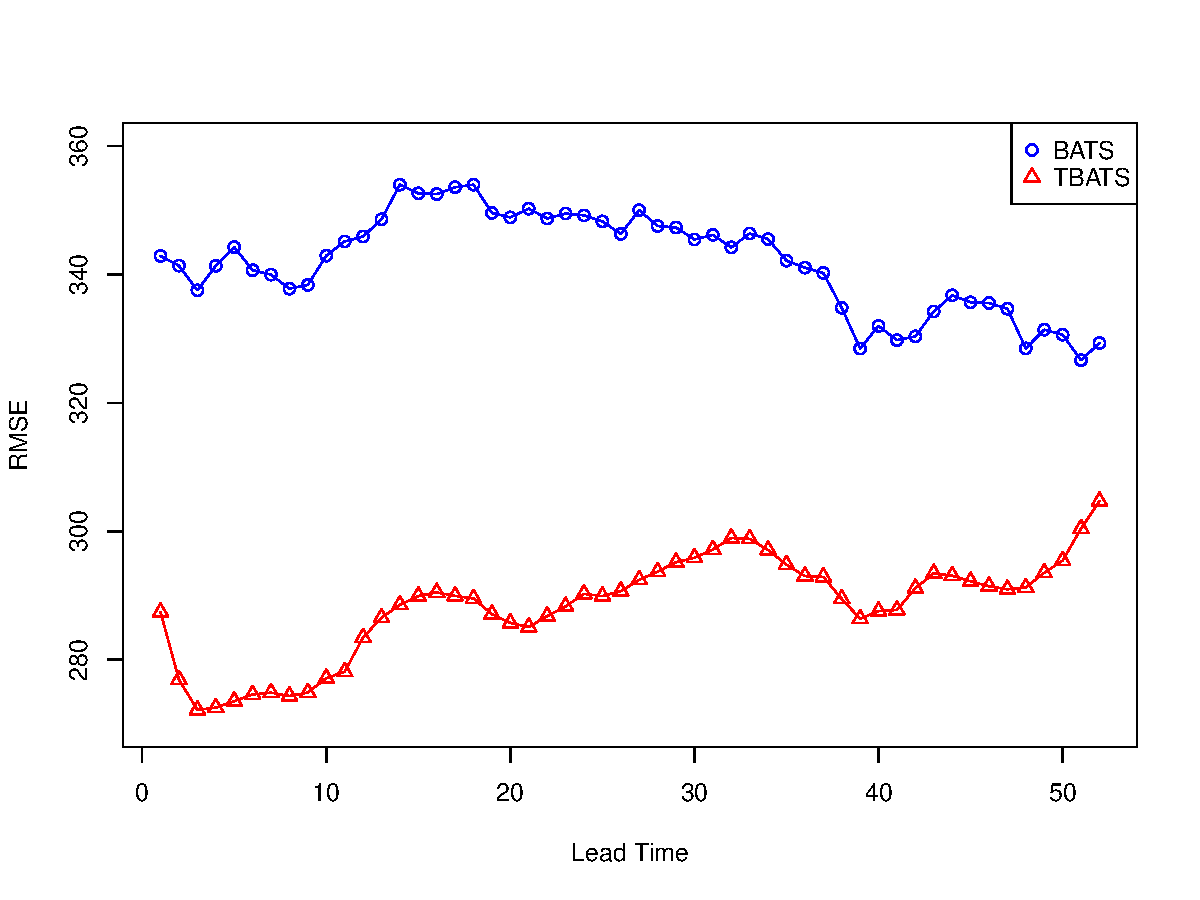
\includegraphics[width=6in,height=3in]{gasRMSE.pdf}
  \caption{Out-of-sample results for the U.S. gasoline data using BATS(1,1,1,0,52) and TBATS(0.6562,0.8035,0,0,\{365.25/7,9\}).}
  \label{fig:gasRMSE}
\end{figure}

\begin{figure}[]
\centering
  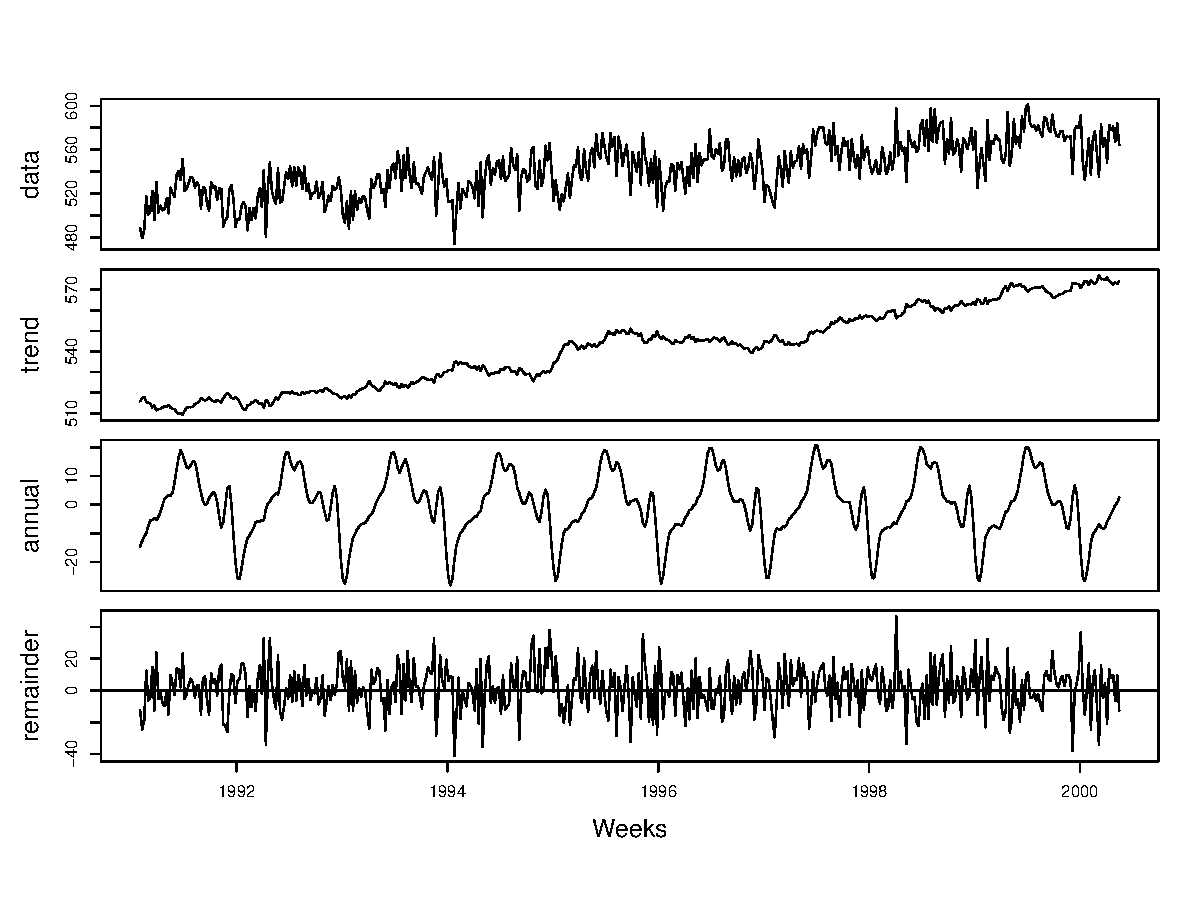
\includegraphics[width=\linewidth,height=4in]{tbatsDecompGas.pdf}
  \caption{Trigonometric decomposition of the U.S. gasoline data. The within-sample RMSE of Box-Cox transformed data was 12.42.}
  \label{fig:tbatsDecompGas}
\end{figure}


\subsection{Application to Call Center Data}
\hspace{4ex}Figure \ref{fig:data} (middle) shows 8 weeks of number of call arrivals on weekdays for every five-minute interval from July 7, 2003, to August 29, 2003. The time series has a daily seasonal pattern with seasonal period $m_1=169$ and a weekly seasonal pattern with seasonal period $m_2=845$. As the trend appears to be close to zero, we omit the growth rate $b_t$. The training set consists of six weeks of data (5070 observations) and the test set consists of two weeks of data (1690 observations). 

The models selected with minimum AIC are BATS(1,NA,2,0,169,845) and TBATS(1,NA,2,\\2, \{169,6\},\{845,4\}), where NA is due to the omitted growth rate. The estimated parameters are shown in Table \ref{table:TBATS} and Table \ref{table:BATS}. The forecasting performances of the two models are shown in Figure \ref{fig:callsRMSE}, where TBATS model has smaller RMSE values than BATS model at all lead times. As with the gasoline dataset, both models have worse forecasting results than the models in the paper.

The trigonometric decomposition of the call center data is shown in Figure \ref{fig:telecRMSE}, where strong daily and weekly seasonal components are exhibited. Both the daily and weekly seasonal patterns are stable, and the trend components is small in magnitude compared to the seasonal components. TBATS model has strong computing advantage against BATS model: the former took 1-2 days to fit, mainly due to \texttt{optim}, while the latter was fitted within an hour. 


\begin{figure}[]
\centering
  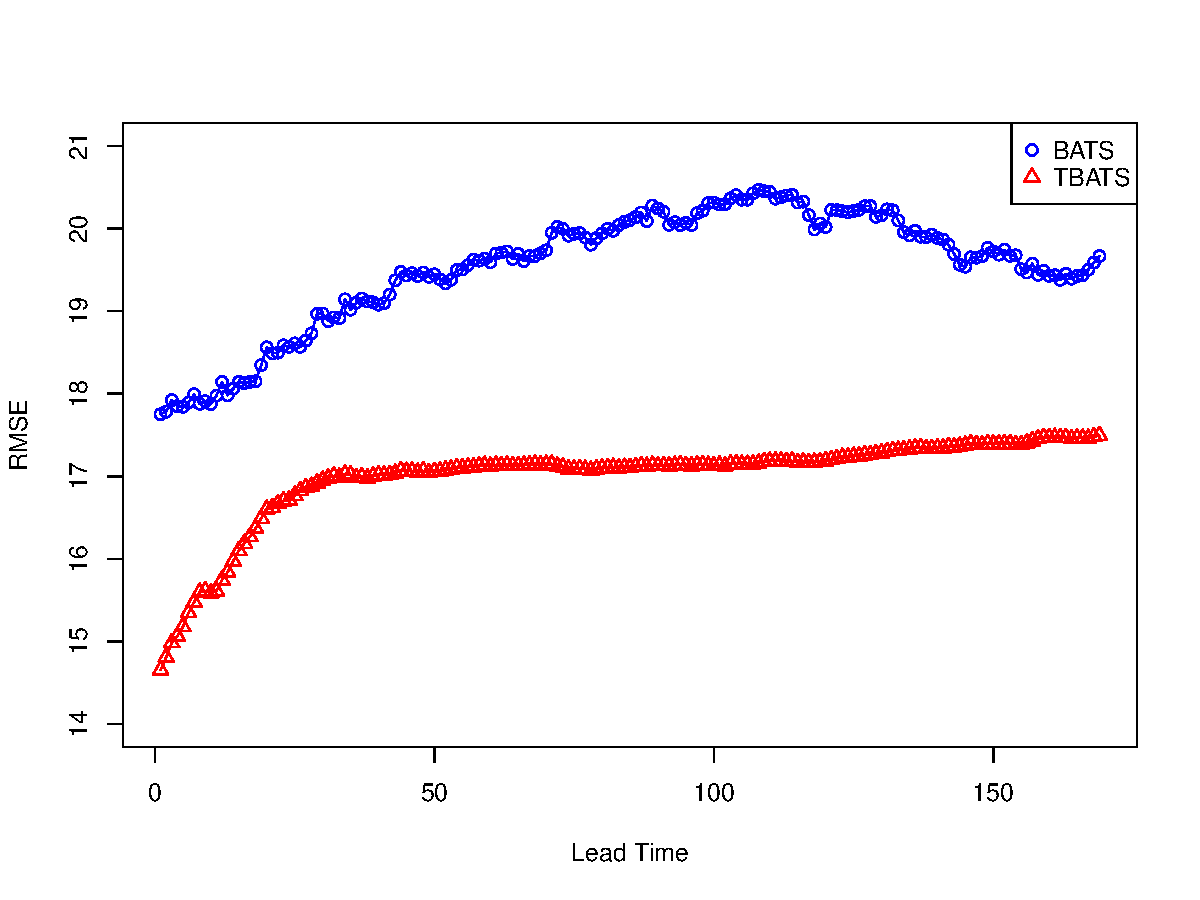
\includegraphics[width=6in,height=3in]{callsRMSE.pdf}
  \caption{Out-of-sample results for the call center data using BATS(1,NA,2,0,169,845) and TBATS(1,NA,2,2,\{169,6\},\{845,4\}).}
  \label{fig:callsRMSE}
\end{figure}

\begin{figure}[]
\centering
  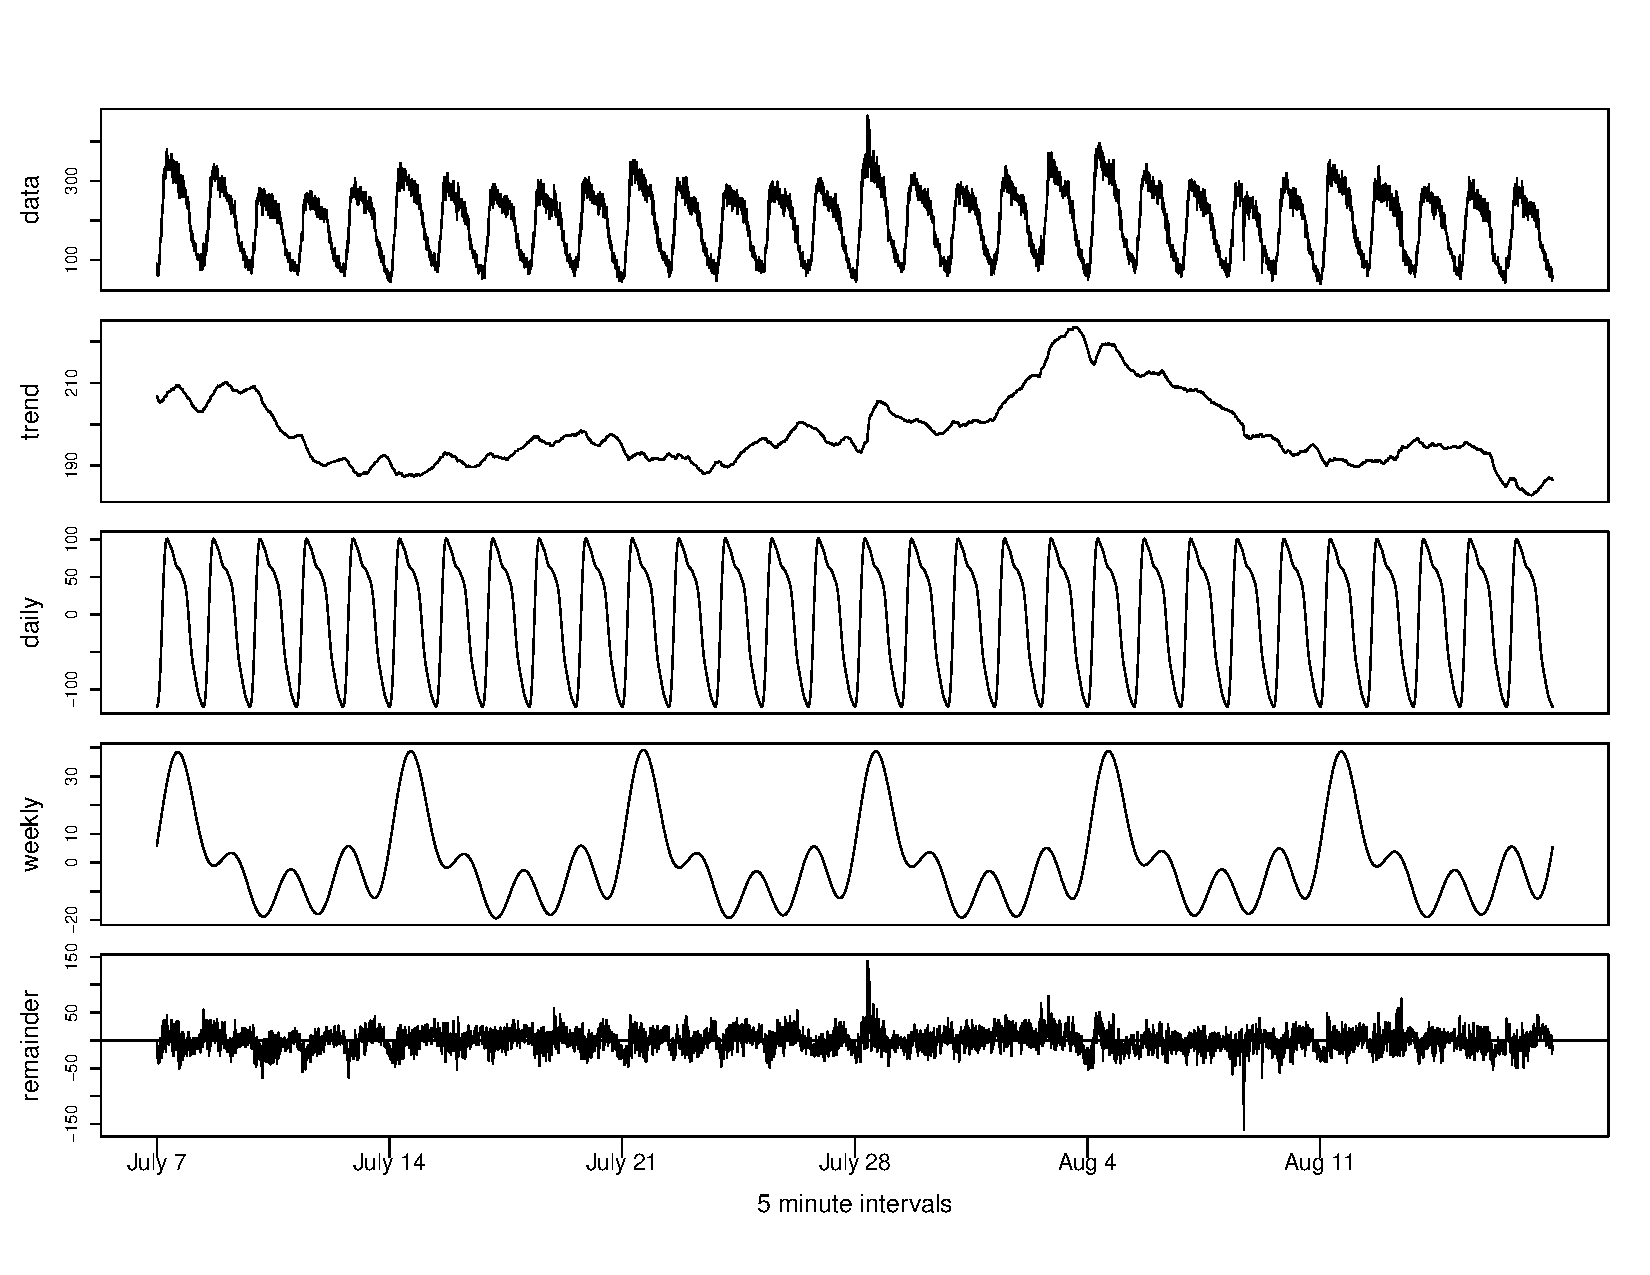
\includegraphics[width=\linewidth,height=5in]{tbatsDecompCalls.pdf}
  \caption{Trigonometric decomposition of the call center data. The within-sample RMSE was 15.28.}
  \label{fig:tbatsDecompCalls}
\end{figure}


\subsection{Application to the Turkey Electricity Demand Data}
\hspace{4ex}Figure \ref{fig:data} (bottom) shows 9 years of daily Turkey electricity demand series from January 1, 2000, to December 31, 2008. Three seasonal components exist with $m_1=7, m_2=354.37, m_3=365.25$. The electricity demand is affected by two Turkish religious holidays which are based on Hijri calendar with period 354.37, and national holidays which are based on Gregorian calendar with period 365.25. The exact dates of holidays are given in Table 3 of \citet{de2011forecasting}. The training set consists of first 6 years of data (2191 observations) and the test set consists of last three years of data (1096 observations). The models selected with minimum AIC are BATS(1,1,5,4,7,354,365) and TBATS(1,1,1,5,\{7,3\},\{354.37,5\},\{365.25,10\}).

Parameter estimates in Table \ref{table:TBATS} and \ref{table:BATS} suggest that Box-Cox transformation is not required for neither BATS or TBATS. The estimated value of $\beta$ is zero in the BATS model with $\phi=1$, which suggests constant growth rate. Forecasts evaluations are illustrated in Figure \ref{fig:tbatsDecompTelec}, where TBATS model performed better than BATS model in the beginning, but got worse as the lead time increased. This is contrary to the paper results, where TBATS model always performs better than BATS model.

The trigonometric decomposition of the Turkey Electricity Demand Data is shown in Figure \ref{fig:tbatsDecompTelec}. The second panel shows an upward trend, and the fifth and sixth panels show the seasonal components based on Hijri calendar and Gregorian calendar, respectively. Hijri seasonal component is more stable than Gregorian seasonal component. Their combined effect is shown in the fourth panel, Hijri and Gregorian seasonal components do not offset each other.

\begin{figure}[]
\centering
  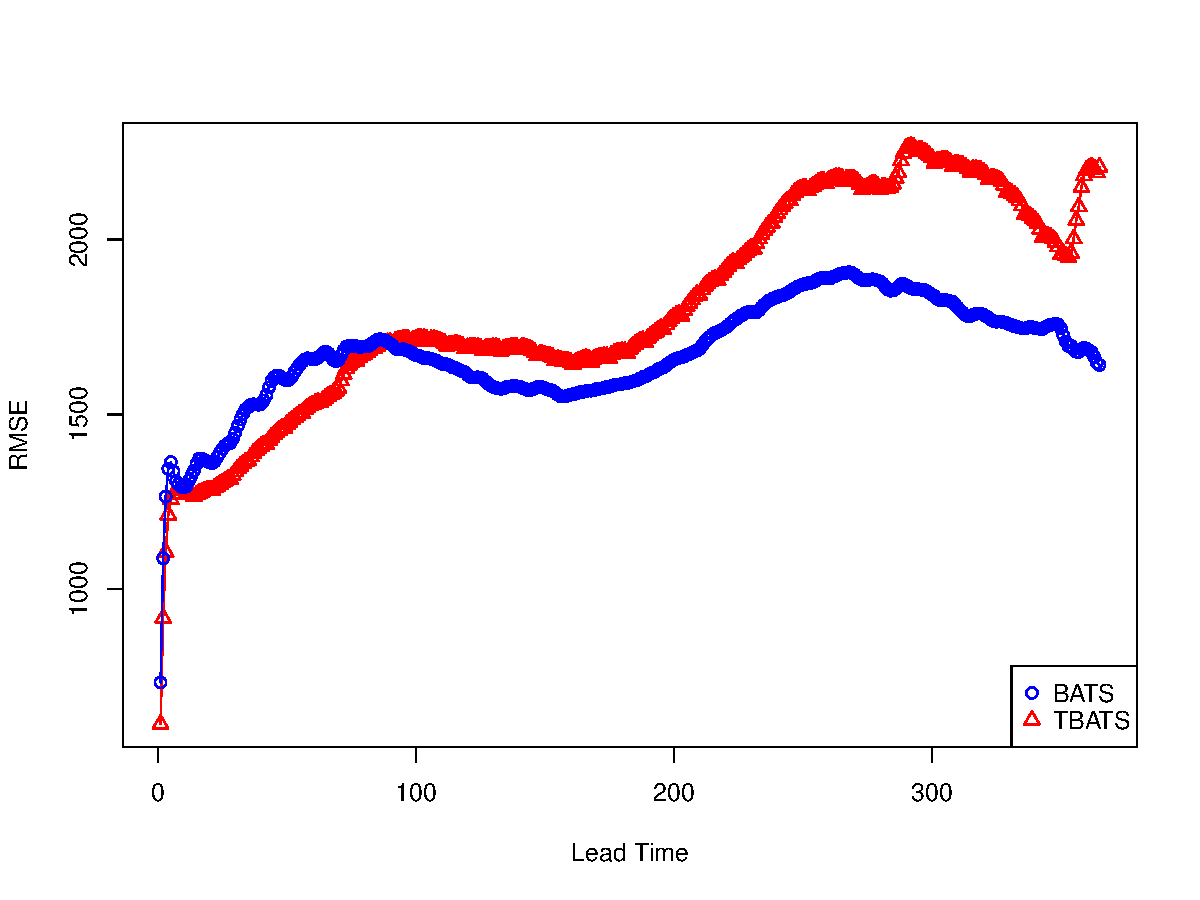
\includegraphics[width=6in,height=3in]{telecRMSE.pdf}
  \caption{Out-of-sample results for the turkey electricity demand data using BATS(1,1,5,4,7,354,365) and TBATS(1,1,1,5,\{7,3\},\{354.37,5\},\{365.25,10\}).}
  \label{fig:telecRMSE}
\end{figure}


\begin{figure}[]
\centering
  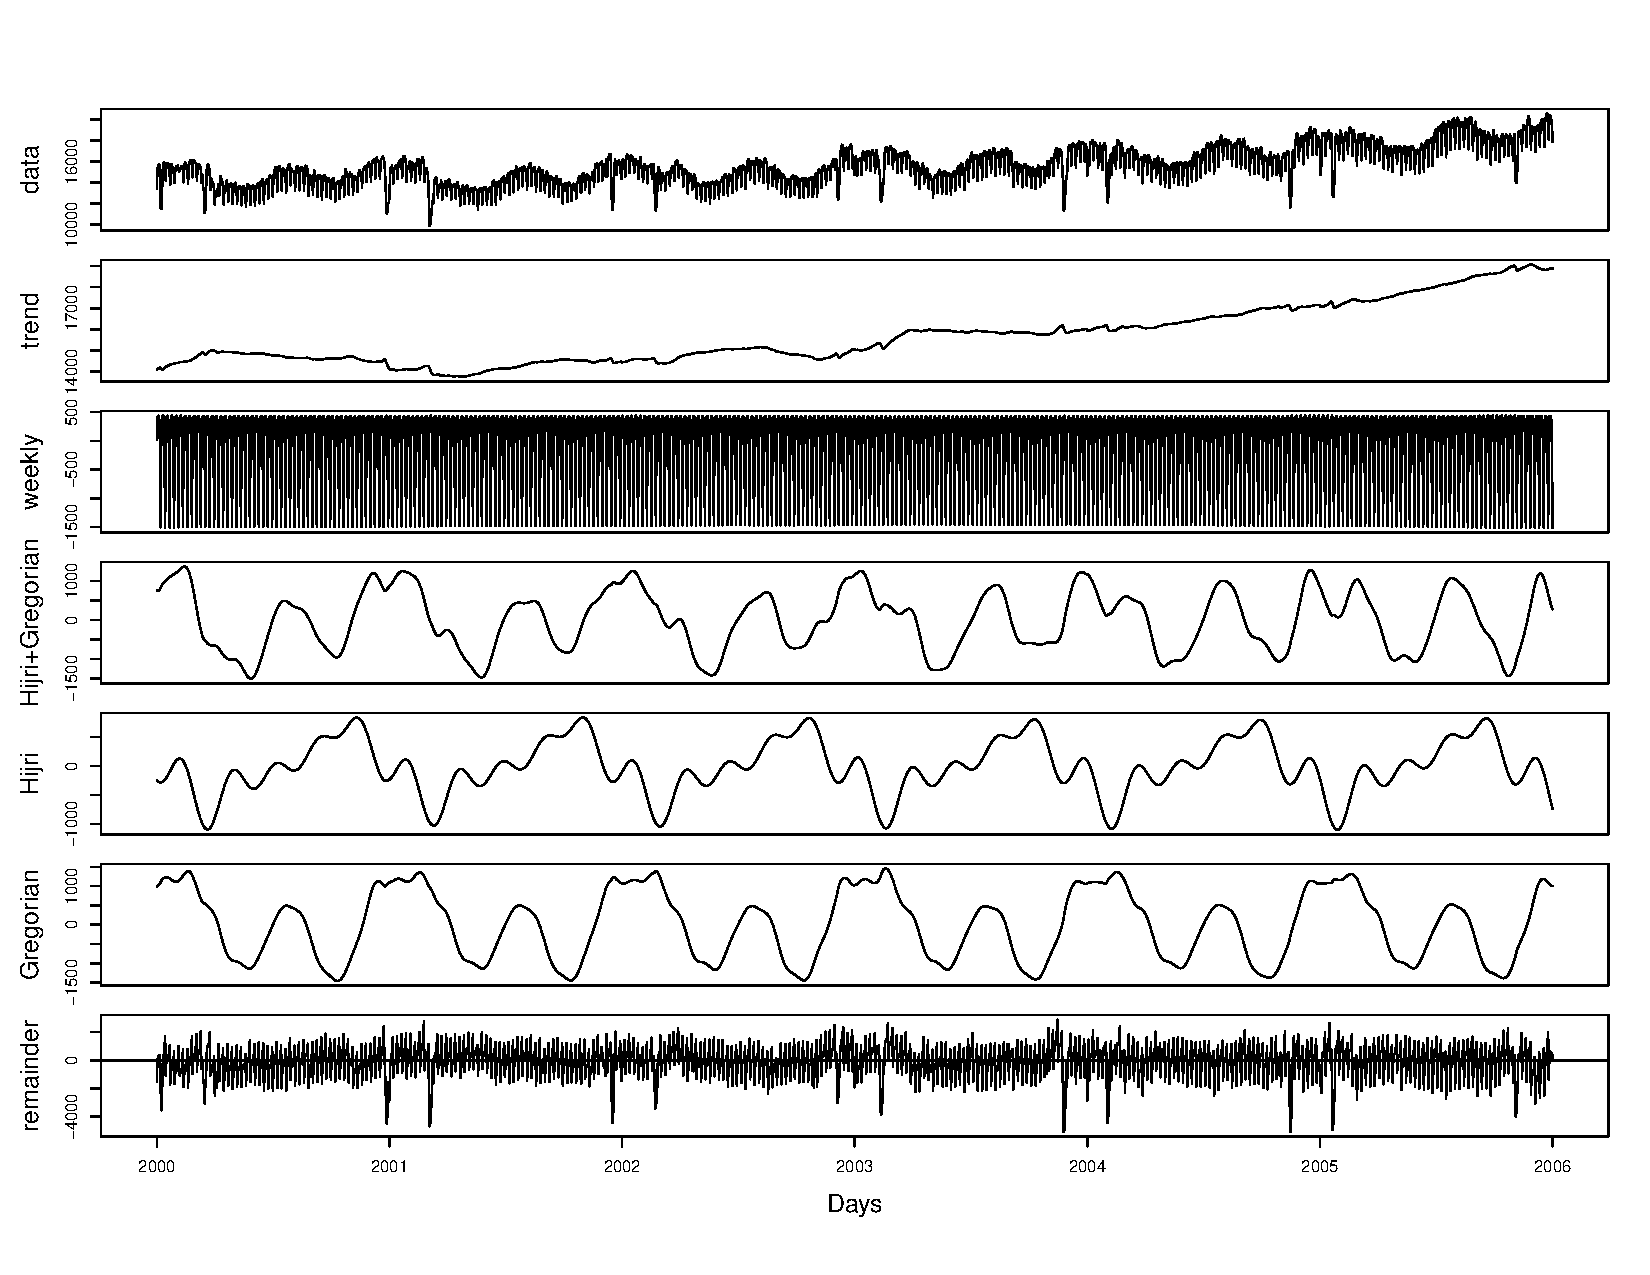
\includegraphics[width=\linewidth,height=6in]{tbatsDecompTelec.pdf}
  \caption{Trignometric decomposition of the Turkey demand data. The within-sample RMSE was 404.03.}
  \label{fig:tbatsDecompTelec}
\end{figure}

\begin{table}[]
\small
\centering
\caption{Number of estimated parameters for each model in each application}
\label{table:number}
\begin{tabular}{l l l l l l l l l l l l l l l l}
\hline \hline
Data & Model & No.parameters \\ \hline
Gasoline & BATS(1,1,1,0,52) & 59 \\
 & TBATS(0.6562,0.8035,0,0,\{365.25/7,9\}) & 26 \\
 Call center & BATS(1,NA,2,0,169,845) & 1022  \\
  & TBATS(1,NA,2,2,\{169,6\},\{845,4\}) & 34  \\
 Electricity & BATS(1,1,5,4,7,354,365) & 752  \\
  & TBATS(1,1,1,5,\{7,3\},\{354.37,5\},\{365.25,10\}) & 58  \\ \hline
\end{tabular}
\end{table}




%\nocite{*}
\clearpage
\newpage
\bibliography{ref}


\end{document}









